\subsection{Search Algorithms}
\label{sec:search}

The underlying algorithms (Negamax, Alpha-Beta pruning, and quiescence search)
were introduced in \cref{sec:preliminaries}. This subsection turns to their
concrete realization in code and to how the individual mechanisms interact in
practice. Particular attention is paid to the two refinements of
this thesis: the move loop is organized as a Principal Variation Search
(\cref{subsec:pvs_implementation}), and previous search trees are resumed
through the persistent transposition table (\cref{subsec:tree_reuse}).

\subsubsection{Search Entry Point and Modes}

The main entry point is \texttt{ChessBot::think()}, which receives the board
together with a \texttt{SearchConstraints} object. The constraints are copied
intentionally and stored inside the engine instance for the duration of the
search. Before searching, the engine
initializes a clean state via \texttt{reset\_search\_state()}, which resets node
counters, selective depth tracking, stop state, and heuristic tables (killer and
history), and also advances the transposition table generation via
\texttt{tt.new\_search()}.

Depending on \texttt{config.mode\_}, the engine selects one of the following
execution strategies:
\begin{itemize}
    \item \textbf{FixedDepth:} the time budget is explicitly disabled
    (\texttt{budget\_ = \{\}}) to prevent time-based termination inside
    \texttt{hard\_stop()}. The engine performs a single root search with the
    requested depth and returns the result.
    \item \textbf{NodeLimit / Infinite:} time-based termination is disabled and
    the engine runs iterative deepening until an external stop condition
    (or the node limit) is hit.
    \item \textbf{Normal / FixedTime (time-managed):} the \texttt{TimeManager}
    initializes a soft and hard deadline from the constraints, and iterative
    deepening runs under these deadlines.
\end{itemize}

This structure keeps the actual search logic independent of UCI parsing and
ensures that all termination behavior is expressed through the constraint object
and the common stop checks.

\subsubsection{Termination and Safety Checks}

All immediate termination decisions are centralized in
\texttt{ChessBot::hard\_stop()}, which is called frequently inside the search
(including quiescence) and combines an external stop flag, the hard time
deadline, and an optional node budget. The exact semantics of these criteria,
and the distinction between the hard deadline and the \emph{soft} deadline that
is only consulted between completed iterations of iterative deepening, are
described in \cref{sec:time_management}.

The stop flag and the node budget are checked at every node, the clock only every
1024 nodes. Reading a monotonic clock costs considerably more than the comparison
it guards, and at the node rates the engine reaches, the resulting imprecision
stays below a millisecond.

As an additional robustness measure, the engine verifies the final move before
returning it. If the selected move is not legal (checked via
\texttt{is\_legal\_move()}), the engine falls back to a legal move
obtained from \texttt{get\_legal\_fallback\_move()}.

\subsubsection{Iterative Deepening Loop}

Time-managed searches run in \texttt{ChessBot::iterative\_deepening(Board\&)}.
The engine starts with a legal fallback move and then performs repeated searches
with increasing depth $d = 1,2,3,\dots$.

For each iteration, a local copy of the current best move is passed into
\texttt{root\_search()}. If the search completes successfully, the resulting move
becomes the new best move and is reported via the UCI \texttt{info} output
(\texttt{print\_info}). If an iteration is aborted (e.g., due to a hard stop),
the loop terminates and the engine returns the best move from the last completed
iteration.

Hard stops are enforced immediately inside the search, while soft stops only
take effect at iteration boundaries (cf. \cref{sec:time_management}).

\subsubsection{Root Search and Core Negamax}

The helper \texttt{root\_search(Board\&, depth, Move\&)} is a thin wrapper that
invokes Negamax with the initial window $[-\infty, +\infty]$ and ply $0$.
The best move is returned through the referenced move parameter, which avoids
additional return-value plumbing and keeps the recursive signature compact.

The core search routine \texttt{ChessBot::negamax(...)} implements a standard
depth-limited Negamax with Alpha-Beta bounds:
\begin{itemize}
    \item If \texttt{depth <= 0}, the search transitions into quiescence search.
    \item At every node, \texttt{hard\_stop()} may terminate the search early.
    \item The routine maintains and updates $\alpha$ during move exploration; a
    cutoff occurs when $\alpha \ge \beta$.
\end{itemize}

To support correct transposition table storage, the implementation stores the
original alpha value (\texttt{ORIGINAL\_ALPHA}) and uses it later to classify the
result as \texttt{EXACT}, \texttt{LOWER\_BOUND}, or \texttt{UPPER\_BOUND}.

\paragraph{Legal Move Handling}
Moves are generated as pseudo-legal moves and filtered by attempting to apply
them with \texttt{board.make\_move(move)}. If \texttt{make\_move} fails (e.g.,
because the move leaves the king in check), the move is discarded. This design
keeps move generation simpler and delegates legality to the make--unmake layer,
which also guarantees that the search only recurses into legal positions.

\paragraph{Terminal Positions}
If no legal move exists, the implementation distinguishes:
\begin{itemize}
    \item \textbf{checkmate:} if the side to move is in check, return a mate score
    of the form $-(MATE - ply)$,
    \item \textbf{stalemate:} otherwise return $0$.
\end{itemize}
Using the current ply in the mate score ensures that faster mates are preferred
and slower mates are avoided.

\subsubsection{Principal Variation Search}
\label{subsec:pvs_implementation}

The move loop inside \texttt{negamax} implements the Principal Variation Search
scheme introduced in \cref{sec:preliminaries}. Instead of searching every move
with the full window $[\alpha, \beta]$, the engine searches only the leading
moves with the full window and verifies all remaining moves with a null-window
search $[\alpha, \alpha + 1]$ (realized as $[-\alpha - 1, -\alpha]$ in the
Negamax formulation). Only if the null-window search indicates that a move can
beat $\alpha$ without already exceeding $\beta$ is the move re-searched with
the full window to obtain its exact score.

The behavior is controlled by two tunable parameters bundled in a
\texttt{PvsConfig} structure:
\begin{itemize}
    \item \texttt{min\_depth} (default $2$): below this remaining depth the
    scout search is skipped entirely and all moves are searched with the full
    window. At shallow nodes the subtrees are so small that the potential
    re-search overhead would outweigh the savings of the null-window search.
    \item \texttt{scout\_after\_move} (default $1$): the first $N$ legal
    moves of a node are always searched with the full window. Move ordering is
    least reliable for the very first moves, so the engine only switches to the
    cheap null-window scout once the presumed principal variation has been
    established.
\end{itemize}

Both parameters are exposed as UCI options (\texttt{PvsMinDepth} and
\texttt{PvsScoutAfterMove}), which allows the scouting behavior to be tuned and
evaluated experimentally without recompiling the engine. The overall structure
of the move loop is summarized in \cref{algo:pvs}.

\begin{algorithm}[ht]
\DontPrintSemicolon
\KwIn{Position $P$, depth $d$, bounds $\alpha, \beta$, legal move counter $n$}
\KwOut{Score of the searched move}

\uIf{$n < \texttt{scout\_after\_move}$ \textbf{or} $d < \texttt{min\_depth}$}{
    $score \gets -\textsc{Negamax}(P, d-1, -\beta, -\alpha)$\tcp*{full window}
}
\Else{
    $score \gets -\textsc{Negamax}(P, d-1, -\alpha - 1, -\alpha)$\tcp*{null-window scout}
    \If{$\alpha < score < \beta$}{
        $score \gets -\textsc{Negamax}(P, d-1, -\beta, -\alpha)$\tcp*{re-search}
    }
}
\Return $score$\;
\caption{Principal Variation Search inside the Negamax move loop.}
\label{algo:pvs}
\end{algorithm}

A subtle but important implementation detail is the interaction with aborted
searches: if a null-window scout is aborted by a hard stop, its score is not
trusted and no re-search is triggered; instead, the abort is propagated upward
so that the iterative deepening loop can discard the incomplete iteration.

\subsubsection{Quiescence Search}
\label{subsec:quiescence_impl}

Quiescence search is implemented in \texttt{ChessBot::quiescence(...)} and is
entered whenever the regular search reaches depth $0$. The function evaluates
the current position via \texttt{eval::evaluate(board)} and then selectively
extends the search by exploring only tactical moves (captures and en-passant).
Non-capturing moves are skipped explicitly. The captures are filtered out of the
generated list before the list is ordered, so the ordering only has to run over
the handful of moves that are actually searched instead of over all of them.

The implementation uses the standard \emph{stand-pat} scheme:
\begin{itemize}
    \item if the static score already exceeds $\beta$, the node fails high,
    \item otherwise $\alpha$ is updated using the static score and improved
    through capture exploration.
\end{itemize}

As with the main search, \texttt{hard\_stop()} is checked inside quiescence to
enforce hard termination constraints consistently.

\subsubsection{Null-Move Pruning}
\label{subsec:null_move_pruning}

In addition to the exact Alpha-Beta framework, the engine applies null-move
pruning as a forward-pruning enhancement of the baseline search. The underlying
observation is that in most positions having the right to move is an advantage:
if a side is allowed to skip its turn (a \emph{null move}) and the resulting
position, searched to a reduced depth, is still good enough to produce a beta
cutoff, then the position is almost certainly too strong for the opponent and the
whole subtree can be pruned without a full-depth search. The technique goes back
to Beal~\cite{beal1989nullmove} and is a standard component of classical engines.

\cref{fig:nullmove} contrasts the two searches involved. The decisive property is
that the reduced search answers a deliberately easier question than the one the
node actually poses. It grants the opponent a free move and still finds the
position too good, which is strong evidence that the node would also survive a
proper search. Unlike Alpha-Beta this is evidence rather than proof, and the
figure also indicates where it breaks down: in zugzwang positions, having to move
is a disadvantage, so passing improves rather than worsens the position and the
inference is invalid. This is the reason for the guard conditions listed below.

\begin{figure}[ht]
\centering
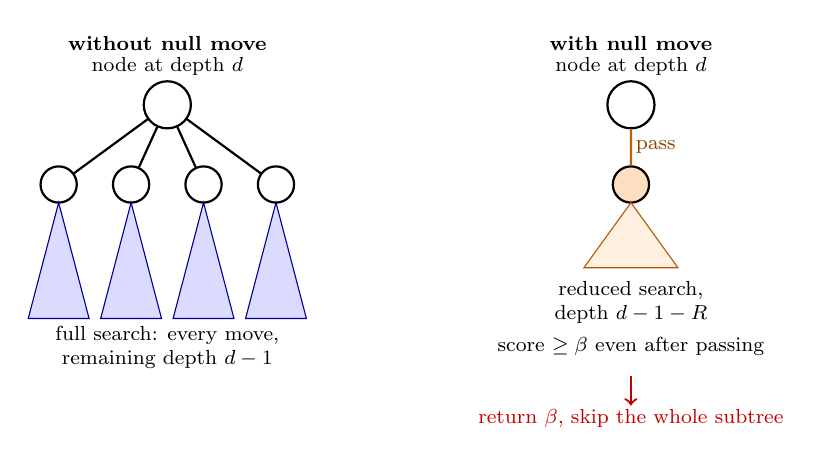
\begin{tikzpicture}[
  scale=0.92, transform shape, font=\small,
  nd/.style={draw, thick, circle, minimum size=6.5mm, inner sep=0pt},
  lbl/.style={font=\footnotesize, inner sep=1.5pt}
]
% ---------------- left: what the node would cost --------------------------
\begin{scope}
  \node[nd] (r) at (2,2.6) {};
  \node[lbl, anchor=south] at (2,2.95) {node at depth $d$};
  \foreach \i/\x in {1/0.5,2/1.5,3/2.5,4/3.5}{
    \node[nd, minimum size=5mm] (m\i) at (\x,1.5) {};
    \draw[thick] (r) -- (m\i);
  }
  \foreach \i/\x in {1/0.5,2/1.5,3/2.5,4/3.5}
    \draw[fill=blue!14, draw=blue!55!black] (\x,1.25) -- (\x-0.42,-0.35) -- (\x+0.42,-0.35) -- cycle;
  \node[lbl, align=center] at (2,-0.75) {full search: every move,\\remaining depth $d-1$};
  \node[font=\footnotesize\bfseries] at (2,3.45) {without null move};
\end{scope}
% ---------------- right: the null-move probe ------------------------------
\begin{scope}[xshift=6.4cm]
  \node[nd] (R) at (2,2.6) {};
  \node[lbl, anchor=south] at (2,2.95) {node at depth $d$};
  \node[nd, minimum size=5mm, fill=orange!25] (P) at (2,1.5) {};
  \draw[thick, orange!75!black] (R) -- node[lbl, right, text=orange!55!black] {pass} (P);
  \draw[fill=orange!12, draw=orange!70!black] (2,1.25) -- (1.35,0.35) -- (2.65,0.35) -- cycle;
  \node[lbl, align=center, anchor=north] at (2,0.22) {reduced search,\\depth $d-1-R$};
  \node[lbl, align=center, anchor=north] at (2,-0.55)
    {score $\geq \beta$ even after passing};
  \draw[->, red!75!black, thick] (2,-1.15) -- (2,-1.55);
  \node[lbl, align=center, anchor=north, text=red!75!black] at (2,-1.55)
    {return $\beta$, skip the whole subtree};
  \node[font=\footnotesize\bfseries] at (2,3.45) {with null move};
\end{scope}
\end{tikzpicture}
\caption{Null-move pruning. Instead of searching every move at full depth (left),
the engine first lets the side to move pass and searches the resulting position
to a reduced depth (right). If the position is still good enough to exceed
$\beta$ despite this handicap, the node is assumed to be beyond the opponent's
reach and the subtree is skipped. The saving is large because the probe is both
shallower and single-branched, but the inference is heuristic: it fails in
zugzwang, where passing would be an improvement rather than a concession.}
\label{fig:nullmove}
\end{figure}

The pruning is performed inside \texttt{negamax}, after the transposition table
probe but before the moves are generated and ordered. The engine plays a null
move via \texttt{board.make\_null\_move()}, searches the resulting position to a
reduced depth $d-1-R$ with a null window around $\beta$ (realized as
$[-\beta, -\beta+1]$ in the Negamax formulation), and restores the position with
\texttt{board.pop\_null\_move()}. If the returned score satisfies
$-\text{score} \ge \beta$, the node fails high and $\beta$ is returned directly.
The number of such cutoffs is tracked in the \texttt{null\_cutoffs} counter for
the experimental instrumentation.

Because null-move pruning is a heuristic rather than an exact technique, it is
guarded by several conditions. The reduced search is only attempted when all of
the following hold:
\begin{itemize}
    \item pruning is enabled and this node was not already reached through a null
    move (\texttt{can\_null}); two consecutive passes are never searched, as they
    correspond to no meaningful line of play,
    \item the node is not the root ($ply > 0$), since the root must always return
    a real best move,
    \item the remaining depth is at least \texttt{min\_depth}; below this the
    reduced search would be too shallow to justify the risk,
    \item $\beta$ is not already a mate score
    ($|\beta| < \texttt{kMate} - \texttt{kMateWindow}$), because a fabricated
    move would distort mate distances,
    \item the side to move is not in check, since passing while in check would
    leave the king en prise,
    \item the side to move still has non-pawn material
    (\texttt{has\_non\_pawn\_material}); in pawn-only endgames zugzwang makes
    passing frequently favourable, which would invalidate the pruning assumption.
\end{itemize}

As in the rest of the search, an aborted reduced search is not trusted: if the
null-move search is terminated by a hard stop, the abort is propagated upward and
no cutoff is derived from the incomplete result. The behaviour is controlled by a
\texttt{NullMoveConfig} structure exposing whether the technique is enabled, the
minimum remaining depth (\texttt{min\_depth}, default $3$), and the depth
reduction (\texttt{reduction}, default $2$). All three are exposed as the UCI
options \texttt{NullMove}, \texttt{NullMoveMinDepth}, and
\texttt{NullMoveReduction}, so the pruning can be toggled and tuned without
recompiling.

\subsubsection{Transposition Table Integration}

The motivation for the table is that the game tree is not, strictly speaking, a
tree. Different sequences of moves frequently lead to the identical position, so
the same node appears many times over at the same depth. A plain recursive search
has no way of noticing this and re-solves each occurrence from scratch, which is
pure duplicated work. \cref{fig:transposition} shows the effect in its smallest
form. Storing results under a hash of the position turns the traversal from a
tree into a directed acyclic graph and lets the second occurrence be answered
from memory. Since the number of such collisions grows with depth, this is one of
the few techniques whose benefit increases rather than decreases as the search
gets deeper, which is also why the same table can be carried across moves
(\cref{subsec:tree_reuse}).

\begin{figure}[ht]
\centering
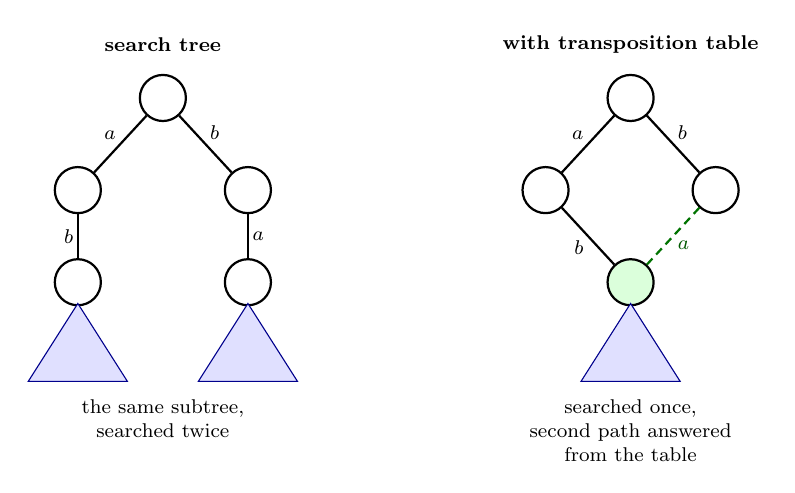
\begin{tikzpicture}[
  scale=0.9, transform shape, font=\small,
  nd/.style={draw, thick, circle, minimum size=6.5mm, inner sep=0pt},
  lbl/.style={font=\footnotesize, inner sep=1.5pt}
]
% ---------------- left: plain tree ----------------
\begin{scope}
  \node[nd] (r) at (2,3) {};
  \node[nd] (x1) at (0.8,1.7) {};
  \node[nd] (x2) at (3.2,1.7) {};
  \node[nd] (y1) at (0.8,0.4) {};
  \node[nd] (y2) at (3.2,0.4) {};
  \draw[thick] (r) -- node[lbl,above left] {$a$} (x1);
  \draw[thick] (r) -- node[lbl,above right] {$b$} (x2);
  \draw[thick] (x1) -- node[lbl,left] {$b$} (y1);
  \draw[thick] (x2) -- node[lbl,right] {$a$} (y2);
  \draw[fill=blue!12, draw=blue!55!black] (0.8,0.1) -- (0.1,-1.0) -- (1.5,-1.0) -- cycle;
  \draw[fill=blue!12, draw=blue!55!black] (3.2,0.1) -- (2.5,-1.0) -- (3.9,-1.0) -- cycle;
  \node[lbl, align=center, anchor=north] at (2,-1.20) {the same subtree,\\searched twice};
  \node[font=\footnotesize\bfseries] at (2,3.75) {search tree};
\end{scope}
% ---------------- right: DAG ----------------
\begin{scope}[xshift=6.6cm]
  \node[nd] (R) at (2,3) {};
  \node[nd] (X1) at (0.8,1.7) {};
  \node[nd] (X2) at (3.2,1.7) {};
  \node[nd, fill=green!14] (Y) at (2,0.4) {};
  \draw[thick] (R) -- node[lbl,above left] {$a$} (X1);
  \draw[thick] (R) -- node[lbl,above right] {$b$} (X2);
  \draw[thick] (X1) -- node[lbl,below left] {$b$} (Y);
  \draw[thick, densely dashed, green!45!black] (X2) --
        node[lbl,below right, text=green!35!black] {$a$} (Y);
  \draw[fill=blue!12, draw=blue!55!black] (2,0.1) -- (1.3,-1.0) -- (2.7,-1.0) -- cycle;
  \node[lbl, align=center, anchor=north] at (2,-1.20) {searched once,\\second path answered\\from the table};
  \node[font=\footnotesize\bfseries] at (2,3.75) {with transposition table};
\end{scope}
\end{tikzpicture}
\caption{Transpositions. Playing move $a$ and then $b$ leads to exactly the same
position as playing $b$ and then $a$, so a plain recursive search explores the
identical subtree twice (left). A transposition table stores the result of the
first visit under a hash of the position, so the second path finds it already
solved and returns immediately (right). Real search trees contain vastly more
such convergences than this minimal example suggests.}
\label{fig:transposition}
\end{figure}

The search consults the transposition table early in \texttt{negamax} via
\texttt{tt.probe(key, depth, alpha, beta, ply, ...)}. A successful probe may:
\begin{itemize}
    \item return an \texttt{EXACT} score,
    \item produce a safe cutoff using stored \texttt{LOWER\_BOUND} or
    \texttt{UPPER\_BOUND} information.
\end{itemize}

In addition, the table provides a stored best move (\texttt{tt\_move}) which is
used for move ordering. Since transposition table entries may be stale or collide,
the implementation verifies the move's legality before using it; illegal TT moves
are discarded.

After searching a node, the result is stored via \texttt{tt.store(...)} together
with the depth, bound type, and the best move found at that node. Mate scores are
encoded in a TT-safe form using the ply (via \texttt{to\_tt\_score} /
\texttt{from\_tt\_score}) so that mate distances remain consistent across
different search depths.

\subsubsection{Search Tree Reuse Across Searches}
\label{subsec:tree_reuse}

The transposition table is not only used within a single search invocation but
also serves as the engine's mechanism for resuming previous search trees. The
table is a member of the engine instance and is deliberately \emph{not} cleared
between searches. When a new search starts, \texttt{reset\_search\_state()}
only calls \texttt{tt.new\_search()}, which advances an internal generation
counter; all stored entries remain accessible. A full \texttt{tt.clear()} is
performed only when the UCI command \texttt{ucinewgame} signals that an
entirely new game begins.

This design directly implements the idea of continuing an earlier computation.
After the engine has played a move and the opponent has answered, the new root
position lies inside the tree that was explored during the previous search.
Probing the persistent table therefore immediately recovers large parts of the
earlier work:
\begin{itemize}
    \item \textbf{Score reuse:} entries stored with sufficient depth yield
    exact scores or safe bound cutoffs without re-searching the corresponding
    subtrees.
    \item \textbf{Move ordering reuse:} stored best moves from the previous
    search guide the move ordering of the new search from the very first
    iteration, which is exactly the situation in which Principal Variation
    Search and Alpha-Beta pruning are most effective.
\end{itemize}

The generation counter implements a soft aging scheme rather than hard
invalidation. The replacement policy prefers overwriting entries from older
generations and entries with lower depth, so stale information gradually
disappears as the game progresses while still being available as long as it is
not displaced. In combination with iterative deepening, this means consecutive
searches behave less like independent computations and more like one continuous
search that is deepened and re-rooted as the game advances.

Keeping the table alive across searches has one consequence that a table cleared
per search does not have: a stored move outlives the position it was generated
for. Since the table is indexed by a truncated key, two different positions can
map to the same entry, and the move handed back then describes pieces that are no
longer where it expects them. Such a move is not merely bad, it is not playable at
all, and applying it would corrupt the board rather than just cost search time.
Every move taken from the table is therefore validated against the current
position before it is used as an answer: it has to be one the move generator
produces here, and it must not leave the own king in check. Moves that come
straight from the generator need no such check, they are pseudo-legal by
construction, so the validation is confined to the few places where a move of
foreign origin enters the search.

\subsubsection{Move Ordering and Heuristics}
\label{subsec:move_ordering}

Move ordering is implemented in \texttt{search::heuristics::order\_moves}.
The ordering score combines several standard heuristics, all of which are
surveyed by Marsland~\cite{marsland1986review}:
\begin{itemize}
    \item \textbf{TT/PV move first:} if a transposition table move exists, it
    receives a large bonus and is sorted to the front.
    \item \textbf{Captures before quiet moves:} captures are prioritized using a
    MVV-LVA-inspired score (most valuable victim / least valuable attacker),
    with a special case for en-passant.
    \item \textbf{Killer moves:} for each ply, the engine tracks up to two quiet
    moves that previously caused beta cutoffs and boosts them in ordering.
    \item \textbf{History heuristic}~\cite{schaeffer1989history}\textbf{:} a 3D
    table indexed by side, from-square, and to-square accumulates bonuses (scaled
    by depth squared) for quiet moves that caused cutoffs, and the accumulated
    score is added during ordering.
\end{itemize}

Killer and history updates are performed only on beta cutoffs and only for quiet
moves. This avoids polluting these tables with captures and ensures that the
heuristics reflect moves that are generally useful for pruning rather than
tactical one-offs.

\subsubsection{Debugging and Instrumentation}

The search provides UCI-compliant reporting via \texttt{print\_info}, including
depth, selective depth, time, nodes, NPS, and either centipawn score or mate
distance (converted from the internal mate representation). Additionally, a
configurable debug facility can emit search health statistics, transposition
table statistics, root move ordering, and principal variation output. This
instrumentation supports the experimental goal of this thesis by making search
behavior observable and reproducible.